\documentclass[11pt]{article}

%-Paquetes
\usepackage{graphicx}
\usepackage{outline}
\usepackage{pmgraph}
\usepackage[normalem]{ulem}
\usepackage[utf8]{inputenc} % Permite el uso de caracteres del Español
\usepackage[T1]{fontenc}

%-Datos de portada
\title{\textbf{Atmósfera Terrestre}}
\author{Jonás Valenzuela Terán\\ \\Actividad 1 - F. Comp.\\Universidad de Sonora}
\date{\oldstylenums{24}/\oldstylenums{01}/\oldstylenums{18}}

%---Make usable space all of page
\setlength{\oddsidemargin}{0in}
\setlength{\evensidemargin}{0in}
\setlength{\topmargin}{0in}
\setlength{\headsep}{-.25in}
\setlength{\textwidth}{6.5in}
\setlength{\textheight}{8.5in}

%---Indention
\setlength{\parindent}{1cm}

\begin{document}
%---Title Page
\maketitle
 
 
%-Documento----------------------------------------------------------

\begin{center}
	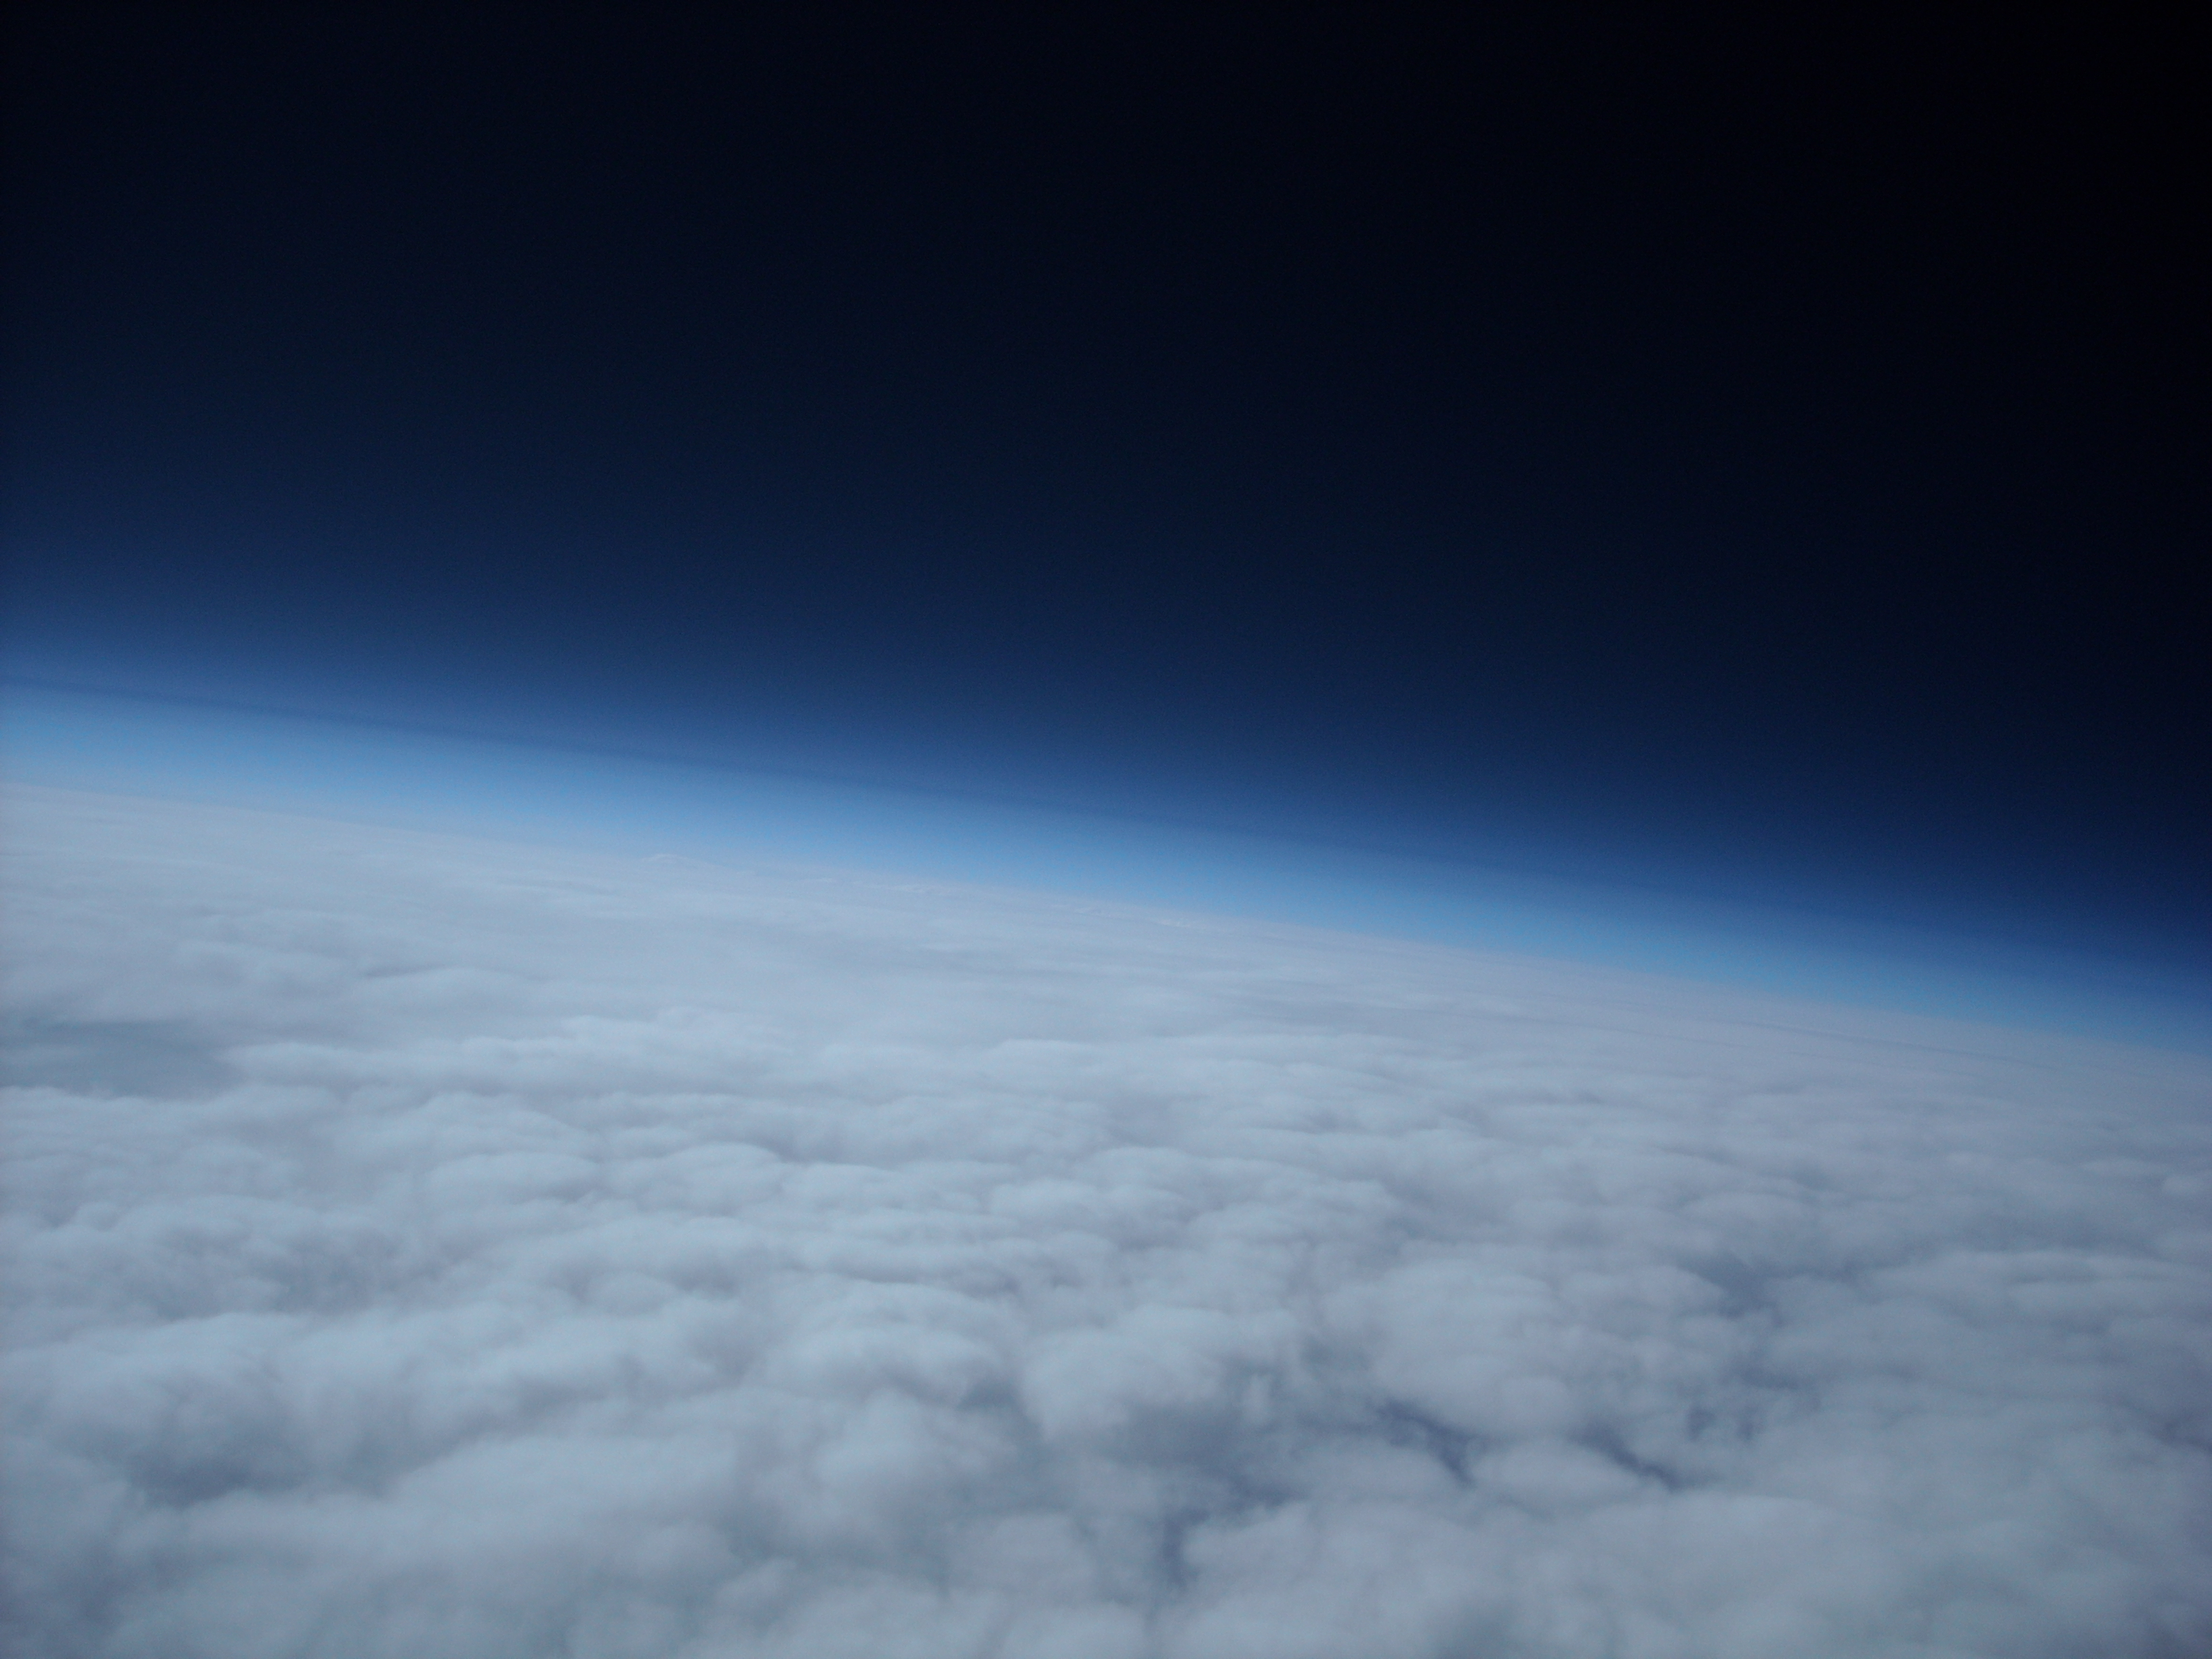
\includegraphics[height=6cm]{atmosfera13.jpg}
	
    By Tecnòlegs de l'IES Bisbal (originally posted to Flickr as DSCN2261) [CC BY-SA 2.0 (https://creativecommons.org/licenses/by-sa/2.0)], via Wikimedia Commons
\end{center}

Esta actividad tiene el propósito de crear un resumen usando el lenguaje \LaTeX, para aprender a usar el lenguaje e incorporarlo a nuestras herramientas de creación de reportes y trabajos. Se resume sobre la atmósfera terrestre, su estructura, divisiones y propiedades.

\section{Introducción}
	La atmósfera de la tierra cubre a todo el planeta, esta compuesta por una numerosa cantidad de combinaciones de gases, comúnmente conocido como aire. Esta capa delgada nos protege de muchas maneras, nos da lo necesario para respirar, mantiene presión constante, absorbe luz ultravioleta y disminuye diferencias de temperatura extremas.
    
    Los seres vivos y el clima ocurre solamente dentro de la troposfera, la atmósfera, tiene una altitud indefinida, haciéndose cada vez menos densa, pero por convención se toma que arriba de 100km de la superficie se considera el espacio exterior. $19.5$



\section{Composición}
	El aire seco de la atmósfera (general) está compuesto principalmente, por nitrógeno (78.084\%), oxígeno (20.946\%), argón (0.9340\%), dióxido de carbono (0.04 \%), neón (0.001818\%), helio (0.000524\%) y metano (0.000179\%). Este puede cambiar dependiendo de la ubicación, capa y clima.


\section{Estructura de la atmósfera}

\begin{center}
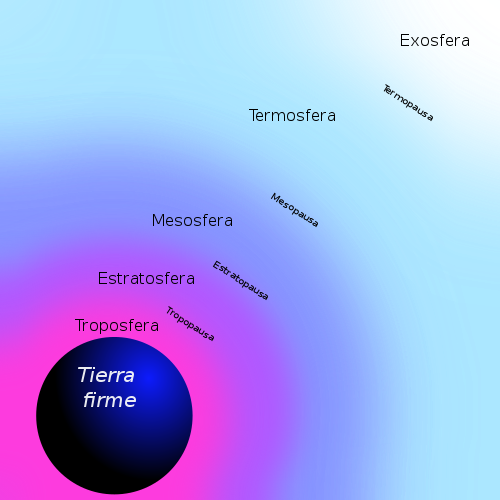
\includegraphics[height=6cm]{terrestre.png}

By Josell7 (Own work) [GFDL (http://www.gnu.org/copyleft/fdl.html) or CC BY-SA 4.0-3.0-2.5-2.0-1.0 (https://creativecommons.org/licenses/by-sa/4.0-3.0-2.5-2.0-1.0)], via Wikimedia Commons
\end{center}
	\subsection{Capas Principales}
    	En general, la presión y la densidad disminuyen cuando aumenta la altura, pero la 		temperatura no tiene un patrón sencillo, el cual nos sirve para distinguir las
      capas principales.
    
    	\subsubsection{Exosfera}
    	Se encuentra entre los 700km y 10,000km, es el lugar de órbita para la mayoría 	 		de los satélites, tiene densidades tan extremadamente bajas que 2 moléculas 			pueden viajar cientos de kilómetros antes de colisionar, por lo que pierde			    el comportamiento de un gas. En esta capa pueden ocurrir auroras boreales,              		compartiéndolas con la termosfera.
        
    	\subsubsection{Termosfera}
        Esta delimitada entre los 80km y 700km, contiene a la ionosfera, su temperatura 		crece con la altitud, hasta los 1500 grados celsius, pero ya que las moléculas se		encuentran a distancias de hasta 1km entre ellas, la temperatura pierde un poco el 		 sentido común que se le da, ya que no conduce mucha energía.
        \subsubsection{Mesosfera}
        Se ubica entre los 50km y 80km de altitud, la temperatura decrece al aumentar la altitud, tanto así que contiene las temperaturas mas bajas del planeta. Es la capa donde la mayoría de los meteoros se deshacen.
        
        \subsubsection{Estratosfera}
        Tiene entre 12 km y 50 km de altitud, contiene la capa de ozono, la temperatura aumenta con la altitud y se considera una atmósfera muy estable ya que es casi completamente libre de nubes y el clima.
	
    	\subsubsection{Troposfera}
        La primera capa de la tierra, va desde la superficie hasta los 12 km, aquí es donde ocurren la mayoría de los fenómenos del clima, casi todo el vapor atmosférico se encuentra en el, todos los aviones comerciales vuelan por esta altitud.
    
    \subsection{Otras capas}
    Dentro de las 5 capas principales mencionadas, se encuentran otras con propiedades interesantes, tales como la capa de ozono que absorbe luz ultravioleta, o la ionosfera que es ionizada por la radiación solar.


\section{Propiedades físicas}

	\subsection{Presión y anchura}
    La presión promedio a nivel del mar es definida como 101325 pascales, la presión y masa de la atmósfera decrece exponencial mente con la altura.
    
    \subsection{Temperatura y velocidad del sonido}
    Las divisiones de la atmósfera se basan principalmente en el comportamiento de la temperatura, ya que este cambia considerablemente, la velocidad del sonido en un gas ideal, depende solo de la temperatura, por lo tanto, varía junto con ella.
    
    \subsection{Densidad y masa}
    La densidad del aire a nivel del mar es aproximadamente 1.2 kg/$m^2$, la densidad al igual que la masa, decrece con la altura, es modelado aproximadamente por la formula barométrica. La masa promedio de la atmósfera es aproximadamente $5$x$10^15$.


\section{Propiedades ópticas}

\begin{center}
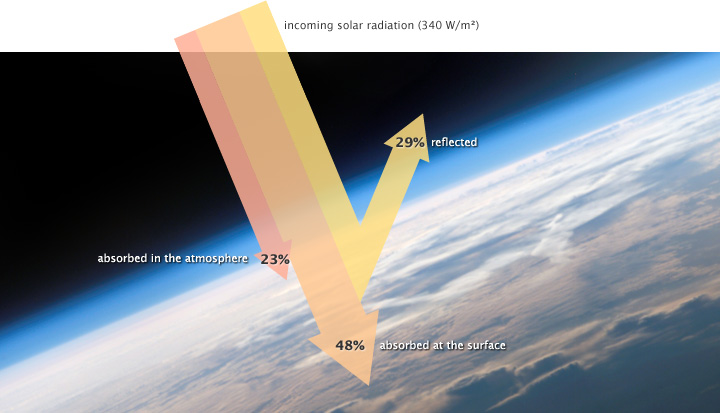
\includegraphics[height=6cm]{NASA.jpg}

By Tecnòlegs de l'IES Bisbal (originally posted to Flickr as DSCN2261) [CC BY-SA 2.0 (https://creativecommons.org/licenses/by-sa/2.0)], via Wikimedia Commons
\end{center}

    La radiación solar es absorbida como energía por la tierra, pero luz de longitud de onda mayores las refleja.
    
	\subsection{Dispersión}
	Cuando la luz pasa por la atmósfera, hace interacción con los gases que atraviesa, cambiando su dirección y disminuyendo su intensidad, es por esto que el cielo cambia de color.
    
    \subsection{Absorción}
    Las moléculas absorben luz de diferentes longitudes de onda, al hacer esto, aumentan su energía, que calienta la atmósfera, pero el proceso inverso ocurre por igual.
    
    \subsection{Emisión}
    Emisión es el proceso inverso de la absorción, las moléculas emiten radiación de una longitud de onda dependiente de su temperatura, por esto, la atmósfera emite luz infrarroja. 
    
    \subsection{Índice de refracción}
    	El índice de refracción ligeramente mayor y cercano a 1, esto depende de la temperatura, puede ocasionar efectos como ver objetos más lejos que el horizonte.

\section{Circulación}

La circulación de la atmósfera es el movimiento del aire a grande escala, por la troposfera y es la manera en que se distribuye el calor. La estructura de la circulación varia con los años, pero en general se mantiene estable ya que es determinado por la rotación de la tierra y la diferencia de radiación solar.

\section*{Bibliografía}
\begin{itemize}
\item (27 de Diciembre, 2017). Atmosphere of Earth. 24 de Enero, 2018, de Wikipedia Sitio web: $https://en.wikipedia.org/wiki/Atmosphere_of_Earth$
\end{itemize}

\section*{Apéndice}


\begin{itemize}
\item  ¿Qué fue lo que más te llamó la atención de esta actividad?

Se me hizo interesante aprender sobre como funciona los diferentes estilos de documento (articulo y reporte) además de como agregar imágenes.

\item  ¿Qué fue lo que se te hizo menos interesante?

No encontré algo particular que no sea interesante o útil

\item  ¿Qué cambios harías para mejorar esta actividad? 

Un texto que involucre un poco más notación matemática

\item  ¿Cuál es tu primera impresión de uso de LATEX?

Es muy formal, funcional y solo se necesita aprender comandos.

\item  ¿El tiempo sugerido para esta actividad fue suficiente? 

Si

\item  ¿Encontraste algún documento o recurso en línea útil que quisieras compartir con los demás?

Si, lo compartí en grupo de redes sociales.

\end{itemize}




\end{document}